% !TeX encoding = UTF-8
% !TeX spellcheck = en_US
% !TeX root = ../presentation.tex

%----------------------------------------------------------------
\begin{frame}{Frame 1}
\frametitle {Frames description}
 
 \begin{columns}
 \begin{column}{0.7\textwidth}
		\begin{itemize}
		\item map
 			 \begin{itemize}
  				\item map is a world fixed frame
 				 \item discrete property make it a poor reference frame for local sensing and acting
  			\end{itemize}
		\item odom
		\begin{itemize}
			\item  pose of robot in the odom frame can drift over time
			\item  useful as an accurate, short-term local reference
		\end{itemize}
	\item base\_footprint
		\begin{itemize}
		\item robot position on the ground
		\item used for object avoidance
		\end{itemize}
	\item base\_link
	\item base\_laser\_front\_link
	\item base\_laser\_rear\_link
	\end{itemize}
\end{column} 
 

\begin{column}{0.4\textwidth}  %%<--- here
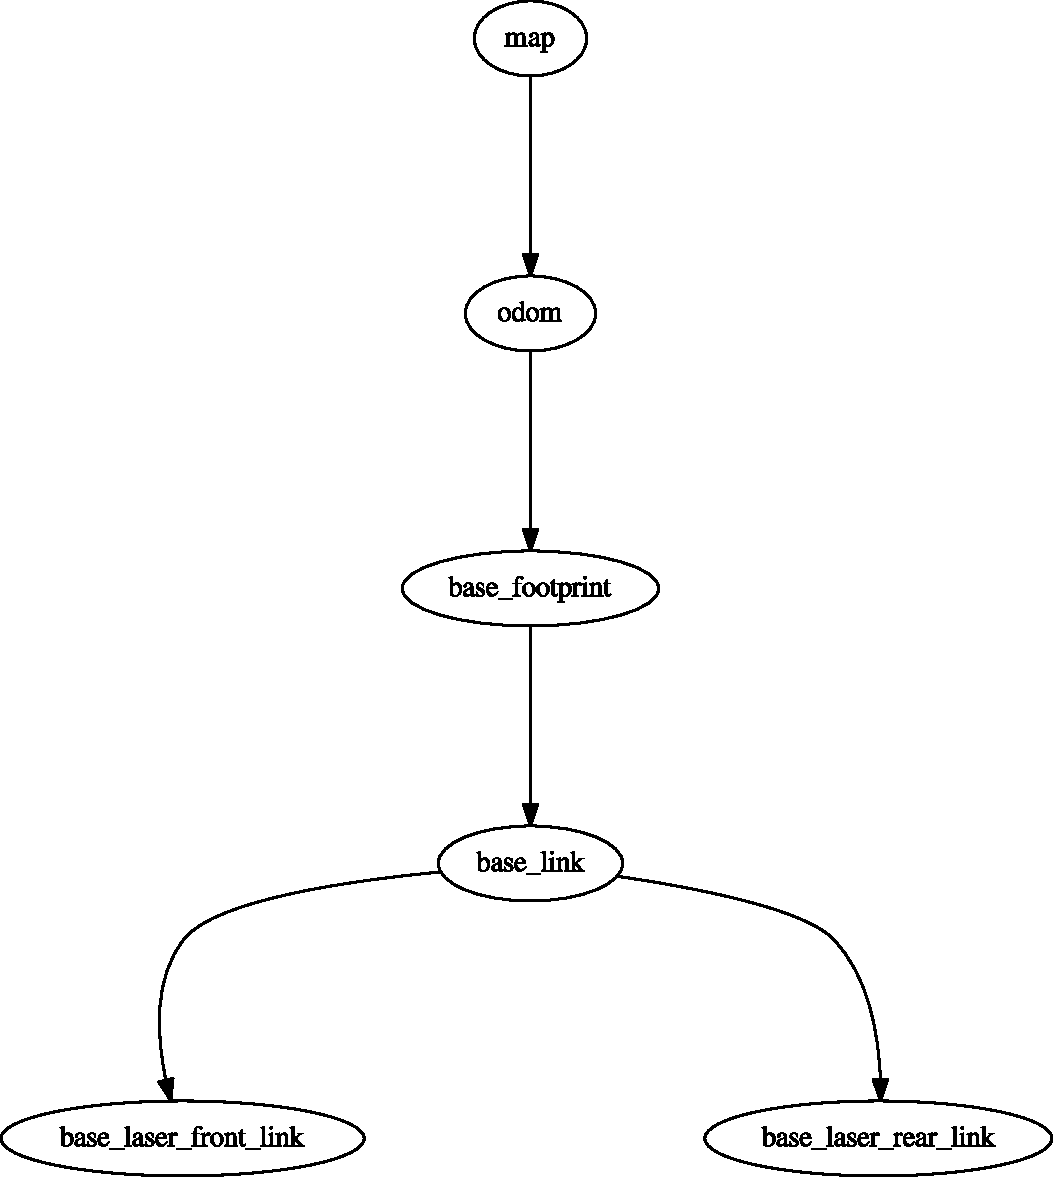
\includegraphics[width=\textwidth]{slides/gfx/frames_cleaned}
\end{column}
\end{columns}

 
\end{frame}